\documentclass[12pt]{article}
\usepackage[utf8]{inputenc}
\usepackage[T1]{fontenc}
\usepackage{cite}
\usepackage{graphicx}
\usepackage{float}
\usepackage[colorlinks]{hyperref}
\hypersetup{
  colorlinks = true,
  linkcolor  = magenta,
  citecolor  = magenta
}
\usepackage[all]{hypcap}
\usepackage{listings}
\usepackage{color}
\definecolor{dkgreen}{rgb}{0,0.6,0}
\definecolor{gray}{rgb}{0.5,0.5,0.5}
\definecolor{mauve}{rgb}{0.58,0,0.82}
\lstset{frame=tb,
  language=Python,
  aboveskip=3mm,
  belowskip=3mm,
  showstringspaces=false,
  columns=flexible,
  basicstyle={\small\ttfamily},
  numbers=none,
  numberstyle=\tiny\color{gray},
  keywordstyle=\color{blue},
  commentstyle=\color{dkgreen},
  stringstyle=\color{mauve},
  breaklines=true,
  breakatwhitespace=true,
  tabsize=3
}

\title{Project Checkpoint: CSE 6730 Project 1}
\author{Chris Dunlap, Allen Koh, Matt May}
\date{Spring 2016}

\begin{document}

\begin{titlepage}
  \maketitle
  \thispagestyle{empty}
\end{titlepage}

\newpage
  \tableofcontents
  \thispagestyle{empty}
\newpage

\section{Problem Statement}
\label{sec:problem}

The efficient evacuation of physical structures is an important problem with a
long history of multi-disciplinary study \cite{zheng2009modeling}. For this
study, we focus specifically on the problem of efficiently evacuating the
area around Bobby Dodd Stadium in Atlanta, GA. Bobby Dodd Stadium, the home of
the NCAA Division-I Georgia Tech Yellow Jackets football team, has a
seating capacity of 55,000 individuals.

\begin{figure}[H]
  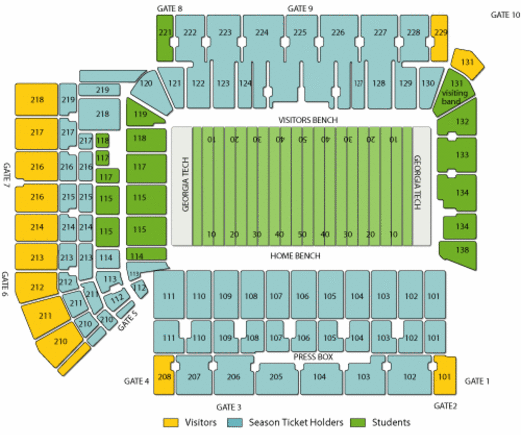
\includegraphics[width=\linewidth,natwidth=521,natheight=435]{stadium_diagram_updated.png}
  \caption{Bobby Stadium Stadium seating chart.}
  \label{fig:polygon}
\end{figure}

Our primary objective in this study is to minimize the pedestrian evacuation
time of the stadium and its surrounding area as attendees leave the area
following a home football game. We do this by taking a parametric approach, in
which we explore the effects of road closures, strategically placed guidance
symbols (i.e., signs), and the ``takeover'' of certain intersections by law
enforcement in promoting an optimal result.

For purposes of this study, we define the system under investigation (SUI) as a
rectangular polygon (Fig. \ref{fig:polygon}) surrounding the stadium. To be
clear, the SUI is defined as the area inside the polygon but outside the
stadium. As pedestrians exit the stadium, they enter the SUI, and as they cross
the boundary of the polygon, they exit it.

\begin{figure}[H]
  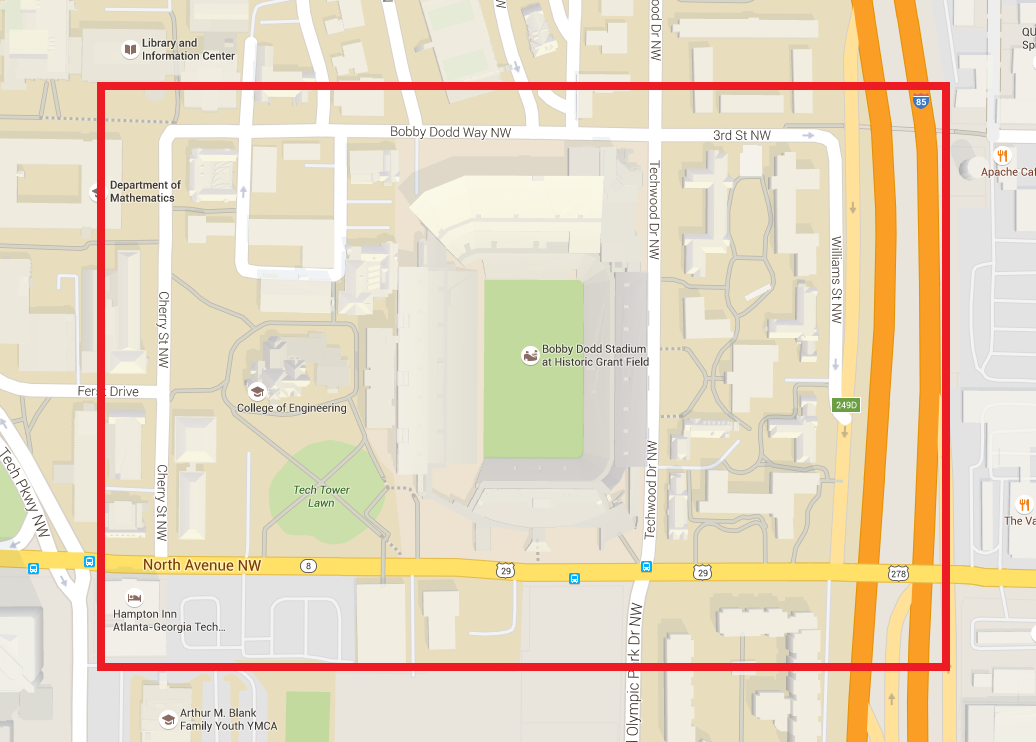
\includegraphics[width=\linewidth,natwidth=1036,natheight=742]{cropped_map.png}
  \caption{The system under investigation.}
  \label{fig:polygon}
\end{figure}

The stadium has 10 ``gates,'' which serve as ingress (pre-game) and egress
(post-game) sites. These serve as the entry points to our simulation. As
pedestrians enter the SUI, they are assigned a destination and then proceed
to their destination by way of pedestrian walking paths (i.e., sidewalks).

\section{Related Work}
\label{sec:literature}

A variety of techniques have been used to model pedestrian movement. Cellular
automata, lattice gas, social force, fluid-dynamic, agent-based, game-theoretic,
and animal experimentation-based approaches have been used
\cite{zheng2009modeling}. As noted by Zheng, Zhong, and Liu
\cite{zheng2009modeling}, models often encounter or attempt to model several
common phenomena: clogging, side-stepping, lane formation, and herding
behavior, among them.

These phenomena manifest themselves in different ways and at different
magnitudes depending on the system being modeled. In one of the early
explorations of 2D cellular automata for simulating traffic flow in the related
domain of vehicular traffic simulation, Biham and Middleton \cite{biham1992self}
note the presence of a sharp
\textit{jamming transition} in which all cars in the simulation transition from
moving at maximal speed to being stuck. Similar effects were noted in
simulations of bi-directional pedestrian movement, with Weifeng, Lizhong, and
Weicheng \cite{weifeng2003simulation} finding that as total pedestrian density
increases, a critical value is reached at which the system transitions into a
jammed state where only a few pedestrians are able to proceed.

In a slightly different take on the problem, Okazaki and Matsushita
\cite{okazaki1993study} modeled pedestrian evacuation using Coulomb's Law, with
actors magnetically moving toward their goals and away from obstacles that would
lead to collisions. In another application of equations of natural phenomena,
Helbing \cite{helbing1998fluid} derived fluid dynamic equations for explaining
the movement of pedestrian crowds, observing phenomena such as the development
of lanes, jamming, and crossing. Helbing \cite{helbing2000simulating} further
notes an explicit ``faster-is-slower'' effect, in which attempting to move faster
results in a lower average speed of leaving at high pedestrian density in
evacuation scenarios.

In a more recent study, Helbing et al. \cite{helbing2005self} use a
``social force'' model, which states that pedestrians operate in some sense
automatically when reacting to obstacles and other pedestrians, applying
strategies that have been learned to be most effective over time. Several
suggestions are made to alleviate the three most common problems in pedestrian
crowds: counterflows, bottlenecks, and intersecting flows. The presence of
strategically placed obstacles are found to actually reduce these negative
phenomena, leading to improved flow.

Building on previous cellular automata-based models, Burstedde et al.
\cite{burstedde2001simulation} introduce a \textit{floor field}, a secondary
grid of cells which underlies the main grid and acts as a substitute for
pedestrian intelligence. These fields can be either static or dynamic, and are
capable of promoting the avoidance of jams, as well as simulating attractive
effects, in which pedestrians are more likely to follow in the paths of
pedestrians ahead of them.

Taking a more algorithmic approach, Fang et al. \cite{fang2011hierarchical} have
designed a modified ant colony optimization (ACO) algorithm for optimizing
pedestrian evacuation, seeking to minimize evacuation time, evacuation distance,
and congestion. Kemloh Wagoum, Seyfried, and Holl \cite{kemloh2012modeling}
utilize an observation principle approach in modeling pedestrian evacuation,
in which pedestrians first observe their environment and then make a final
decision on strategy based on obtained data.

There are several takeaways from the literature described above that have
potential applicability to the model at hand. First, on the topic of modeling
pedestrian walkways, several papers focused on either a single passageway,
enclosed areas with obstacles (walls, pillars, etc.), or evacuation from a
room with a single doorway. However, modeling walkways as a undirected graph
\cite{fang2011hierarchical} seems feasible given the problem at hand, where
there are multiple pathways one can take to get to a single destination. In
papers where cellular automata was utilized, the median size of each cell on the
walkway was 0.4m\textsuperscript{2}
\cite{blue2001cellular,burstedde2001simulation,weifeng2003simulation}.

Second, on the topic of pedestrian modeling, multiple walking speed techniques
were used, ranging from a constant speed of 1 m/s \cite{weifeng2003simulation}
or 1.3 m/s \cite{burstedde2001simulation}, to using a distribution resembling a
step function \cite{blue2001cellular} or a Normal distribution
\cite{klupfel2005models}. In either distribution, the median walking speed was
also approximately 1.3 m/s. For reaction to stimuli, 0.3 seconds was utilized
\cite{burstedde2001simulation}, which was one time step in that particular
simulation. Incorporation of opportunistic side-stepping was done
\cite{blue2001cellular}, in addition to using least-cost algorithms for
establishing the path a pedestrian would like to take
\cite{fang2011hierarchical}. In the context of cellular automata, analyzing a
given pedestrian's cell's neighbors in either a 4-connected
\cite{weifeng2003simulation} or 8-connected fashion
\cite{burstedde2001simulation} to decide in which direction the pedestrian would
like to walk for the next time step was utilized. This, coupled with a dynamic
floor field \cite{burstedde2001simulation} to factor in long-distance forces,
could be utilized.

Finally, simulation execution practices were also gleaned. Care must be taken
to do parallel-based updating to avoid sequential updating from interfering with
underlying model execution \cite{blue2001cellular}. The practice of using
a deterministic model running with randomized initial conditions has precedent
\cite{biham1992self}. Finally, to achieve statistical significance, 20 runs per
configuration has been used \cite{blue2001cellular}.

\section{Conceptual Model}
For our simulation, we utilize a 2-dimensional cellular automata (CA)-based
approach. We construct a discrete time-stepped model, in which the simulation
clock advances by a fixed interval every time step. We utilize a stochastic
(probabilistic) approach, in which the output of each individual simulation
run is a random variable. Thus, multiple simulation runs will be performed and
statistical analysis will be used to provide confidence levels in our results.

\subsection{Inputs}
The primary input to our simulation model is a stream of football game attendees
(i.e., pedestrians) exiting Bobby Dodd Stadium following a home football game.
For purposes of modeling this input stream, we assume pedestrian interarrival
time at the stadium gate boundary is a homogeneous stochastic process that
follows a Poisson distribution. If the average rate of people exiting the
stadium is known, the Poisson distribution will give a probability distribution
of when the next person will exit within a set interval of time, independent
of the last person who exited the stadium. As pedestrians arrive at the gate
boundary, they enter the SUI.

In addition, we select each pedestrian's target destination and walking
speed at random. For selecting a target destination, we sample from
an empirical distribution. For determining a walking speed for each pedestrian,
we sample from a distribution previously referenced in the literature by Blue
and Adler \cite{blue2001cellular} (5\% fast walkers (4 cells/time step), 90\%
standard (3 cells/time step), 5\% slow (2 cells/time step)).

Pedestrians in our model can be considered a consumer entity class
\textit{Pedestrian} with attributes which will be set and updated during the
course of our simulation. Table \ref{table:ped} provides an overview of the
attributes of the \textit{Pedestrian} class.

\def\arraystretch{1.5}
\begin{table}[hb!]
  \centering
    \begin{tabular}{p{0.3\linewidth}p{0.6\linewidth}}
     \hline
     Attribute & Description \\
     \hline
     Current        & \textit{Node} object corresponding to the current
                      location of the pedestrian. \\
     Destination    & \textit{Node} object (see Table \ref{table:node})
                      corresponding to the final destination of the
                      pedestrian. \\
     TargetNext     & The desired next node to move to in the pedestrian's
                      shortest path to his destination, as computed by
                      Dijkstra's algorithm. \\
     Speed          & Walking speed, formulated in grid cells traversed per
                      time step. \\
     EgressComplete & A boolean value. This value is false when the pedestrian
                      has not yet egressed, and true when egress is complete. \\
     \hline
    \end{tabular}
    \caption{Attributes of the \textit{Pedestrian} entity class.}
  \label{table:ped}
\end{table}

New instances of the \textit{Pedestrian} class are created and initialized
as pedestrians exit the stadium.

\subsection{Output}
For each simulation run, when all pedestrians were evacuated from the SUI we
determined the simulation to be complete. As this is a stochastic simulation,
the output results must be interpreted as samples of a random process.

At the conclusion of a series of simulation runs for a given set of parameters,
we compute an average of the total egress duration across all runs from that
series. More formally, the average egress time $E_{avg}$ for $n$ simulation runs
can be represented as:

\begin{equation}
E_{avg} = \frac{1}{n}\sum\limits_{i=1}^n d_i
\end{equation}

where $d_i$ is the total egress duration of the $i$th simulation run. This
output can be considered a derived scalar output variable (DSOV). We then
define the optimal parameter strategy to be the set of parameters $P$ that
give the the minimum value of $E_{avg}$.

\subsection{Content}

\subsubsection{Approach}
Pedestrians exit the stadium from one of four potential exits. To build the
simulation space, we overlay a 2-dimensional cellular automata grid on a map of
the SUI. We model this space as a weighted graph, a type of graph in which each
graph edge is assigned a weight corresponding to the spatial distance between
the two nodes \cite{west2001introduction}. Note that in this
section, the terms ``cell'' and ``node'' are used interchangeably.

As pedestrians exit the stadium (and thus enter the SUI), they are
probabilistically assigned one of the graph’s destination nodes.  When a
pedestrian reaches a destination node, that constitutes them exiting the SUI.
Destination nodes are chosen based on their spatial meaning when overlaid on a
map of the SUI, and constitute one of three possible classes: on-campus housing
(dormitories), parking lots, or the North Avenue Metropolitan Atlanta Rapid
Transit Authority (MARTA) station.

Each node in the graph is a member of a \textit{Node} class, which
has attributes as shown in Table \ref{table:node}.

\def\arraystretch{1.5}
\begin{table}[hb!]
  \centering
    \begin{tabular}{p{0.3\linewidth}p{0.6\linewidth}}
     \hline
     Attribute & Description \\
     \hline
     NodeID      & Unique identifier for the node. \\
     XCoordinate & X-coordinate of the node on the 2-dimensional grid. \\
     YCoordinate & Y-coordinate of the node on the 2-dimensional grid.
                   (Note: for purposes of this simulation, the y-axis is
                    inverted.) \\
     Paths       & A dictionary (hash map) relating each possible destination
                   to the NodeID of the next node in the shortest path as
                   determined by Dijkstra's algorithm. \\
     Neighbors & Array of \textit{Node} objects corresponding to nodes that are
                 one edge away from the node. \\
     Available	& Boolean value indicating whether the node is available for a
                  pedestrian (true) or not available (false). \\
     NodeType   & Enumeration of the type of node, corresponding to its
                  spatial significance. The NodeType can be one of four
                  possibilities: sidewalk, road, SUI entrance, or SUI exit. \\
     \hline
    \end{tabular}
    \caption{Attributes of the \textit{Node} class.}
  \label{table:node}
\end{table}

As part of the simulation initialization, the node and edge information is
populated. For each node in the graph, we pre-compute the least-cost path to
every possible destination node $N_d$. In general, we can compute the shortest
path between any given node $N_i$ and destination node $N_d$ using Dijkstra's
well-known algorithm \cite{dijkstra1959note}. In our simulation, we use a
publicly available Python implementation of Dijkstra's algorithm
\cite{eppstein-dijkstra}. A hash map \textit{Paths} attribute of each node
stores the next node in the least-cost path to each destination.

At each time step, a pedestrian occupying a given node $N_i$ uses the
\textit{Paths} attribute to identify the next desired cell to walk towards given
their destination node $N_d$. This drives the pedestrian’s instinct to move
toward their destination, based strictly on the shortest distance walk from
their current position to $N_d$.

This concept of pre-computing and saving shortest-path data is known as creating
a static floor field (that is, a floor field that does not change as the
simulation progresses). However, a given pedestrian must decide where to move
in light of other pedestrians and other modeled factors. Such factors do change
with time, and requires the use of a dynamic floor field
\cite{burstedde2001simulation}.

The chosen implementation of the dynamic floor field is to be determined.
However, the static floor field will return the next node desired based on the
shortest path; due to the 8-connected nature of the nodes this corresponds
to a specific direction of travel spatially (for example, North or North East).
Thus, it is reasonable to also consider directions adjacent to the “shortest
path” direction when deciding a pedestrian’s next move (for example, a “shortest
path” direction of East would yield adjacent directions of North East and
South East).

It will likely occur that more than one pedestrian will decide to pursue the
same node in a given time step. In such cases, a probabilistic approach is taken
to resolve this conflict (since only one pedestrian can occupy a cell at a
time), depending on their respective walking speeds. If the walking speeds are
the same, each pedestrian will get an equal chance of getting the desired node.
However, if there is a disparity, pedestrian(s) featuring higher walking speeds
will have a higher chance of getting the desired node, and pedestrian(s)
featuring lower walking speeds will have a lower chance of getting the desired
node.

\subsubsection{Parameters}

To optimize the egress of everyone exiting the stadium in our SUI, there are
several parameters that can be altered. The first parameter is closing certain
streets or intersections meant for vehicular traffic and making them for use by
pedestrians only (i.e.,
roads become sidewalks). The second is having traffic police take over certain
intersections to control the pedestrian flow (i.e., overrule traffic lights).
The third is placing signs along the sidewalk to direct pedestrians to walk a
certain direction to their destination. The optimal time for everyone to exit
the stadium and the SUI could be a combination of the three parameters.
For example, directing pedestrian traffic to an intersection that is closed to
all vehicles or controlled by a police officer is a combination that is likely
to produce better results than only directing pedestrians to a regular
crosswalk.

To simulate these parameters, in addition to a \textit{Node} class, there is
also an \textit{Intersection} class, which has attributes as shown in Table
\ref{table:intersection}.

\def\arraystretch{1.5}
\begin{table}[hb!]
  \centering
    \begin{tabular}{p{0.3\linewidth}p{0.6\linewidth}}
     \hline
     Attribute & Description \\
     \hline
     IntId & Integer value. A unique identifier for the intersection. \\
     Nodes & Array of \textit{Node} objects corresponding to nodes
             that are part of this intersection. \\
     IsOpen  & Boolean value indicating whether the intersection is open
             for pedestrian access (true) or not open (false). \\
     \hline
    \end{tabular}
    \caption{Attributes of the \textit{Intersection} class.}
  \label{table:intersection}
\end{table}

To model intersections where vehicles are allowed to pass, the nodes in the
intersections are assigned to a pre-defined intersection. The intersection
is therefore made up of a group of nodes. To simulate the crosswalk opening and
closing, the nodes will be either forced closed or available for pedestrians to
occupy them. If the road is closed and vehicles are passing, then no nodes in
the intersection will be available for pedestrians. The duration of
intersection closure can be determined stochastically or by the number of
pedestrians waiting for the crosswalk to open.

One parameter in the simulation that can be modified is determining which
intersections will be completely closed to vehicles and always available for
pedestrian use. To model this case, all nodes in that intersection will behave
in the same way as the nodes that make up the sidewalk. There will be no need to
create an intersection object for that intersection. On the other hand, if there
is an intersection that is closed off for pedestrians and only available for
vehicular traffic, then the initial creation of nodes will not include that
intersection - there will be no nodes at that intersection as no pedestrian can
ever occupy those nodes.

If there are pedestrians that need to cross an intersection, but the
intersection is closed, then the pedestrians will not be able to advance to
their next node. This will cause a list of pedestrians to stay in their
current node until the crosswalk opens up (i.e., queue). Once that occurs, then
the pedestrians can continue to their next nodes.

\subsubsection{Random Numbers}
To model the egress of the stadium, we take a stochastic (probabilistic)
approach. In the context of a computer simulation, this necessitates the use of
a pseudorandom number generator.

For our simulation, we use the Lehmer random number generator
\cite{payne1969coding}, also known as the Park-Miller random number generator
\cite{park1988random}. For verification of the generator, we performed
100,000 iterations of a chi-square test procedure in which 1,000 samples were
drawn from the random number generator. For each iteration, we placed each
sample into one of 100 bins, forming a histogram. We then computed the
chi-square statistic, namely:

\begin{equation}
{\chi}^2=\sum_{i=1}^{n} \frac{(O_i - E_i)^2}{E_i}
\end{equation}

where ${\chi}^2$ is the chi-squared statistic, which asympotically approaches
a ${\chi}^2$ distribution, $O_i$ is the count of observations of type $i$,
and $E_i$ is the expected count of observations of type $i$. We determined the
chi-square critical value for 99 degrees of freedom and a $p$-value of 0.05 to be
123.225. Experimentally, our generator failed to pass the chi-square test 4.95\%
of the time over 100,000 iterations, allowing us to not reject the null
hypothesis that our random number generator produces uniformly distributed
random numbers with 95\% certainty.

\subsection{Assumptions and Simplifications}
We make a number of assumptions and simplifications in constructing our
simulation model.

Firstly, our simulation is simplified by focusing only on
\textit{pedestrian} traffic, avoiding the inclusion of vehicular traffic which
could be significant in a football game evacuation scenario.

We also assume the stadium to be at or near full seating capacity of 55,000
individuals. While the mean empirical value of football game attendance at
Bobby Dodd Stadium is somewhat lower than 55,000, the choice
of 55,000 allows us to ``stress test'' our model by simulating the upper bound.

We assume that pedestrians stay on sidewalks and obey traffic lights, as the
inclusion of other types of pedestrian behaviors would likely add complexity
to the model without yielding much additional value. We also assume that main
roads such as North Avenue remain open to vehicular traffic, avoiding a more
unrealistic simulation that would be possible if all roads could be closed.

In the realm of our ``updating rule'' which specifies the next cell for a given
pedestrian to travel to in the simulation, we assume that pedestrians are
following a shortest-path approach. While logical, this may be an
oversimplification, as pedestrians (particularly from the home team) may follow
more indirect paths to their destinations following a victory.

We make the assumption that all pedestrians will be traveling to one of three
possible classes of destinations - local housing, MARTA, or a parking facility.
While an important simplification, it is likely true in reality that pedestrians
may be traveling to other destinations as well, such as social venues. It is
also likely that some percentage of pedestrians may not evacuate the area for
an extended time period, as they sit idle while waiting for friends or planning
their destination in an ad-hoc manner.

We assume the stochastic processes in this simulation to be homogenous
stochastic processes, which can be defined as stationary stochastic processes
where the random variables $X = X_1, X_2, ..., X_n$ are independent and
identically distributed. While not always realistic in the context of
simulation model-building, we do believe this assumption to be reasonable in
the context of this simulation.

There are inherent simplifications in the choice of a cellular automata-based
simulation approach. Specifically, it is assumed that each individual travels
a constant distance per time step through the simulation. Nevertheless, we
attempt to mitigate this simplification by drawing the speed for each
individual from a probability distribution, which does introduce some
variation, albeit only on an individual-to-individual basis.

\section{Description of Simulation Software}

\subsection{Architecture}
In generating our simulation, we take an object-oriented design approach. We use
the Python programming language for our implementation.

Distinct types of entities in our simulation are represented as
\textit{classes}. For interacting with these classes, we define a number of
methods that function as their public interfaces. It should be noted that while
we may define explicit ``getter'' and ``setter'' methods in our conceptual model,
the Python programming language provides these interfaces on declared object
attributes without the need to provide explicit method definitions in code.

\subsection{Interfaces}

\subsubsection{User Interface}

To run our simulation, first ensure Python 2.7 is installed on the testing
machine. Python's matplotlib module will also need to be installed for
visualization purposes. If visualization is not needed, it can be turned
off by setting the \textit{Visualization} option to False in the driver program,
\textit{driver.py}.

If Python and the matplotlib module are installed, you can simply enter the
\textit{code} subdirectory and run the following at a Unix command prompt:

\begin{lstlisting}
  $ python driver.py
\end{lstlisting}

The output will initially state that a preprocessing step is being performed
to prepare the simulation. Then, the actual simulation will automatically begin.
Pedestrians will be created and will begin moving toward their destinations. As
they do, the number of ``active pedestrians'' remaining in the SUI will be
displayed at every time step.

To use our simulation in a less rote manner, we have provided a simple interface
by which a user can easily use our software. First, the user creates a
\textit{Grid} object, which is initialized from a maximum number of rows,
maximum number of columns, node file, edge file, and type map giving
translations between integer node types (such as SUI entrance, SUI exit,
sidewalk, and road). An optional file in \textit{pickle} format can contain
previously produced shortest path information.

The node file should be in a CSV format, of the form:

\begin{lstlisting}
  cell_x, cell_y, pixel_x, pixel_y, meters_x, meters_y, node_type
\end{lstlisting}

where cell\textunderscore x and cell\textunderscore y correspond to $x$ and $y$
coordinates in a 2D-grid space. pixel\textunderscore x, pixel\textunderscore y,
meters\textunderscore x, and meters\textunderscore y translate the $x$ and $y$
coordinates into pixel space and physical space, respectively. The
node\textunderscore type is an integer value that specifies whether the node
is a sidewalk (1), road (2), SUI entrance (3), or SUI exit (4) node.

The edge file should also be in a CSV format, of the form:

\begin{lstlisting}
  node_a_id, node_b_id, edge_weight
\end{lstlisting}

where the node ids refer to zero-based line indices in the node file. In other
words, if the node file contained two rows, such as:

\begin{lstlisting}
  1,4,4,16,4,16,2
  2,6,8,24,8,24,2
\end{lstlisting}

A corresponding edge file might look as follows:

\begin{lstlisting}
  0,1,7.000
\end{lstlisting}

where $0$ refers to the node in the first line of the nodes file, and $1$ refers
to the node in the second line.

The type map should be a dictionary, with string keys that are human-readable
descriptions of node types, and integer values that correspond to %node_type
in the node file.

Once the grid is created, it is passed to the \textit{Simulation} constructor,
along with a parameter dictionary with options such as the number of pedestrians
that should be simulated, and whether the visualization engine will be enabled.

A typical driver program might look as follows:

\begin{lstlisting}
# driver.py
from grid import Grid
from simulation import Simulation

# Specify the max number of rows and columns in the grid.
max_rows = 66
max_cols = 139

# Create a type map mapping human-readable node types to integer ids.
type_map = { "sidewalk": 1, "crosswalk": 2, "entrance": 3, "exit": 4 }

# Create a grid object that contains the underlying nodes and path information.
grid = Grid(max_rows, max_cols, "vertices.csv", "edges.csv", type_map)

# Set up a simulation object.
simulation = Simulation(grid, {"num_pedestrians": 500, "visualization": True})

# Run the simulation.
simulation.run()
\end{lstlisting}

\subsubsection{Pedestrian Class Interfaces}
For simulating pedestrian movement, we define a \textit{Pedestrian} class as
shown in Table \ref{table:pedestrian_methods}. Pedestrians are initialized with
an entrance node to the SUI, as well as a destination node and speed. They then
traverse the nodes in the shortest path toward their destination node. Once
they have reached a node with an \textit{exit} NodeType, the
SetEgressComplete() method is called for the pedestrian with an argument of
true, alerting the simulation that the pedestrian has finished the simulation.
Once there are no pedestrians in the simulation remaining with the
EgressComplete attribute set to false, the driver program breaks from the main
simulation loop and the program exits.

\def\arraystretch{1.5}
\begin{table}
  \centering
    \begin{tabular}{p{0.5\linewidth}p{0.5\linewidth}}
     \hline
     Method & Description \\
     \hline
     Move(NewNode) & Takes one argument: a \textit{Node} object. When called,
                     marks the node set to \textit{Current} as unavailable,
                     sets the \textit{Current} attribute to NewNode,
                     and marks the NewNode object as unavailable. \\
     GetCurrentNode() \newline SetCurrentNode(CurrentNode) & Returns or sets
                        the current node that the pedestrian is occupying. \\
     GetDestinationNode() \newline SetDestinationNode(DestNode) & Returns or
                        sets the destination node for the pedestrian. \\
     GetTargetNext() \newline SetTargetNext(TargetNext) & Returns or
                       sets the target next node for the pedestrian in the
                       shortest path to his destination. \\
     GetEgressComplete() \newline SetEgressComplete(Complete) & Returns or
                        sets the current egress status of the pedestrian. True
                        once the pedestrian has exited the SUI, and false
                        otherwise. \\
     \hline
    \end{tabular}
    \caption{Methods of the \textit{Pedestrian} class.}
  \label{table:pedestrian_methods}
\end{table}

\subsubsection{Node Class Interfaces}
We define a \textit{Node} class as shown in Table \ref{table:node_methods}.
Nodes are the primary abstraction for the resource entities in the simulation,
which are sidewalks and roads. Nodes have several key attributes defined that
can be retrieved and set. Among them, the Neighbors attribute specifies all the
nodes that are one degree away from the node object. The Neighbors attribute is
then used to populate the Paths attribute for the node, which is a hash map
that gives the next node in the shortest path to each possible destination node
in the simulation. We precompute the Paths attribute for every node in the
graph prior to beginning the simulation. This precomputation step needs only
be repeated when a parameter change occurs that alters the underlying node
structure or availability.

The GetNextNode() method of the Node class provides the next node in the
shortest path for a given destination. When a pedestrian lands on a given node,
this method is utilized to then provide the pedestrian with his next location
in the following time step.

\def\arraystretch{1.5}
\begin{table}
  \centering
    \begin{tabular}{p{0.5\linewidth}p{0.5\linewidth}}
     \hline
     Method & Description \\
     \hline
     GetAvailable() \newline SetAvailable(Bool)  & Gets or sets the current
                        value of the \textit{Available} attribute for the node.
                        If the setter, must be a boolean true or false. \\
     GetNextNode(DestinationNode) & Takes one argument: destination
                                    \textit{Node} object. Returns the next
                                    \textit{Node} object for the pedestrian to
                                    advance to based on the pedestrian’s final
                                    destination. \\
     GetPaths() \newline SetPaths(Paths) & Returns or sets the Paths attribute
                of the node, which is a hash map that gives the next node in
                the shortest path to each possible destination node in the
                simulation. \\
     GetNeighborNodes() \newline SetNeighborNodes(ListNodes) & Returns or sets
                        the Neighbors attribute of the node, corresponding to
                        the nodes one edge length away. If the setter, takes
                        one argument: list of \textit{Node} objects. \\
     GetNodeType() & Returns the NodeType Attribute of the node. \\
     GetNodeID() & Returns the NodeID Attribute of the node. \\
     \hline
    \end{tabular}
    \caption{Methods of the \textit{Node} class.}
  \label{table:node_methods}
\end{table}

\subsubsection{Intersection Class Interfaces}
Within our simulation, we utilize a number of intersections that are
parametrically closed and opened. Thus, we define key methods for the
\textit{Intersection} class in Table \ref{table:intersection_methods}.

Intersections are used to limit the rate of flow of pedestrians through the SUI,
increasing the reality of the simulation. As an intersection contains one or
more nodes, when an intersection is closed, all the nodes within it are
closed to additional pedestrian traffic. Pedestrians currently in the
intersection as it closes are able to exit the intersection and continue
walking, but no new pedestrian traffic is allowed into the intersection.

In our initial simulation model, we have not yet explored the effects of
the intersections, but nevertheless present code for our intersection
abstraction in \textit{intersection.py}.

\def\arraystretch{1.5}
\begin{table}
  \centering
    \begin{tabular}{p{0.5\linewidth}p{0.5\linewidth}}
     \hline
     Method & Description \\
     \hline
     OpenMe()  & When called, sets the \textit{Available} attribute to
                 true for every node in its \textit{Nodes} array. Sets the
                 \textit{Open} attribute for the intersection to true. \\
     CloseMe() & When called, sets the \textit{Available} attribute to
                 false for every node in its \textit{Nodes} array. Sets the
                 \textit{Open} attribute for the intersection to false. \\
     GetNodes() & Returns the list of \textit{Node} objects that are part of the
                  intersection. \\
     SetNodes(ListNodes) & Takes one argument: list of \textit{Node} objects.
                           Sets the \textit{Node} objects that make up the
                           intersection. \\
     \hline
    \end{tabular}
    \caption{Methods of the \textit{Intersection} class.}
    \label{table:intersection_methods}
\end{table}

\section{Final Notes}
It should be noted that all of the authors contributed equally to this work.
From a testing perspective, our simulation model has been tested primarily in
a Mac OS X environment - specifically, OS X 10.11.3 with Python 2.7.

Thanks are due to the TAs and instructor for their assistance with our many
questions.

\clearpage
\bibliography{template}{}
\bibliographystyle{plain}
\end{document}
